\documentclass[xcolor=dvipsnames,aspectratio=169,t]{beamer}
  % t means frames are vertically centered to the top
\usepackage{slides-header}
\title{Least-Squares Problems and Best-Fit Lines}

\begin{document}
\maketitle

\begin{frame}{Inconsistent Linear Systems}
  
  Consider solving $A\x=\b$.
  \begin{itemize}
    \item If the system is consistent, then $\b$ is in $\Col A$.
    \item If the system is \alert{inconsistent}, then $\b$ is \alert{not} in $\Col A$.
  \end{itemize}
  \bigskip
  
  \pause
  As a consolation prize, let's find $\hat\x$ such that $A\hat\x$ is the \colorb{closest} vector in $\Col A$ to $\b$; that is, 
  \[ \| \b-A\hat\x \| \le \| \b-A\x \| \text{ for all $\x$ in $\R^n$.} \]
  Such a sol'n $\hat\x$ is called a \alert{least-squares solution}
  since $\hat\x$ minimizes $\|\b-A\x\|=\|\z\|=\sqrt{\sum \z_i^2}$.
  \bigskip
  
  \pause
  Let $\hat\b=\proj_{\text{Col }A} \b$.
  Then $\hat\b$ is the \colorb{closest} vector in $\Col A$ to $\b$,
  and $A\hat\x=\hat\b$ is \alert{consistent}.
  \bigskip
  
  \pause
  We know how to do each of these steps:
  \begin{itemize}
    \item Compute $\hat\b=\proj_{\text{Col }A} \b$. (How?)
    \item Solve $A\hat\x=\hat\b$.
    \pause
    \hspace*{15em} But there is a \alert{simpler} way!
  \end{itemize}
\end{frame}


\begin{frame}{Least-Squares Solutions}
\medskip
  
  We wish to find \alert{least-squares solutions} $\hat\x$ to $A\x=\b$.
  \medskip
  
  Such least-squares solutions satisfy $A\hat\x=\hat\b$, where $\hat\b=\proj_{\text{Col }A} \b$.
  \bigskip
  
  \pause
  By the \colorb{Orthogonal Decomposition Theorem}, $\z=\b-\hat\b$ is orthogonal to $\Col A$.
  
  Thus, $\z=\b-A\hat\x$ is orthogonal to each column $\a_j$ of the matrix $A$.
  \begin{align*}
    \a_j \cdot (\b-A\hat\x) &= 0 \text{ for each $j$.} \\
    \a_j^T (\b-A\hat\x) &= 0 \text{ for each $j$.} \\
    \onslide<3->{
    A^T (\b-A\hat\x) &= \mathbf{0}.
    }
  \end{align*}
  
  \pause
  Rearranging, we have that \vspace*{-2.6em}
  
  \[ \hspace*{-1em} (A^T A) \hat\x = A^T\b. \]
  \vspace*{-3.1em}
  
  \hfill These are called the \alert{normal equations}.%
  \medskip
  
  \pause
  \begin{theorem}
  The set of least-squares solutions of $A \x = \b$ is given by the solutions of the \alert{normal equations}.
  \end{theorem}
\end{frame}

\begin{frame}{Example}
\smallskip

  Find the least-squares solutions of $A\x=\b$, where
  $A = \begin{bmatrix} 4 & 0 \\ 0 & 2 \\ 1 & 1 \end{bmatrix}$
  and 
  $\b = \begin{bmatrix} 2 \\ 0 \\ 11 \end{bmatrix}$.
  \medskip
  
  \pause
  Notice that 
  $\small \left[\begin{array}{cc|c} 4 & 0 & 2\\0 & 2 & 0\\1 & 1 & 11\end{array}\right]
  \xrightarrow{\text{RREF}}
  \left[\begin{array}{cc|c} 1 & 0 & 0\\0 & 1 & 0\\0 & 0 & \alert{1} \end{array}\right]$.
  Hence the system is \alert{inconsistent}.
  \vspace*{2em}
  
  \pause
  \begin{columns}[T]
  \column{.35\textwidth}
  We solve the \alert{normal equations}:
  \column{.5\textwidth}
  \vspace*{-1.5em}
  \begin{align*}
    A^T A\x & =A^T\b. \\
    \begin{bmatrix} 17 & 1 \\ 1 & 5 \end{bmatrix} \x &=
    \begin{bmatrix} 19 \\ 11 \end{bmatrix}
    \hspace*{3em} \text{one sol: } \hat\x=\begin{bmatrix} 1 \\ 2 \end{bmatrix}.
  \end{align*}
  \end{columns}
  \bigskip
  
  \pause
  \blue{Compare}:
  \smallskip
  
  \quad G--S: $\small \left\{ \begin{bmatrix}4 \\ 0 \\ 1 \end{bmatrix},
    \begin{bmatrix} -4/17 \\ 2 \\ 16/17 \end{bmatrix} \right\}$, \quad
  $\hat\b=\proj_{\Span\{\v_1,\v_2\}} \b 
    = \textstyle \left( \frac{\b \cdot \v_1}{\v_1 \cdot \v_1} \right) \v_1
    + \textstyle \left( \frac{\b \cdot \v_2}{\v_2 \cdot \v_2} \right) \v_2
  =\small \begin{bmatrix} 4 \\ 4 \\ 3 \end{bmatrix} = A \hat\x.
  $
  
\end{frame}


\begin{frame}{Unique solution to the Least-Squares Problem}
  \smallskip

  \begin{theorem}
  The set of least-squares solutions of $A \x = \b$ is given by the solutions of the \alert{normal equations} 
  \vspace*{-.75em}
  
  \[ A^TA \x = A^T \b.\]
  \end{theorem}
  \smallskip

  \pause
  \begin{theorem}
  Let $A$ be an $m \times n$ matrix. The following statements are \blue{logically equivalent}:
  \bb[(a)]
  \ii The equation $A \x = \b$ has a \alert{unique} least-squares solution for each $\b$ in $\R^m$.\smallskip
  \ii The columns of $A$ are \alert{linearly independent}.\smallskip
  \ii The matrix $A^T A$ is \alert{invertible}.\smallskip
  \ee
  When these statements are satisfied, the least-squares solution $\hat\x$ is given by
  \vspace*{-.75em}
  
  \[ \hat\x = (A^TA)^{-1}A^T \b .\]
  \end{theorem}
\end{frame}


\begin{frame}{Best-Fit Line}
  \medskip
  
  Suppose we have $n$ data points $(x_1,y_1),\ldots,(x_n,y_n)$.
  What is the line that \alert{best fits} this data?
  
  \begin{columns}[T]
  \column{.5\textwidth}
    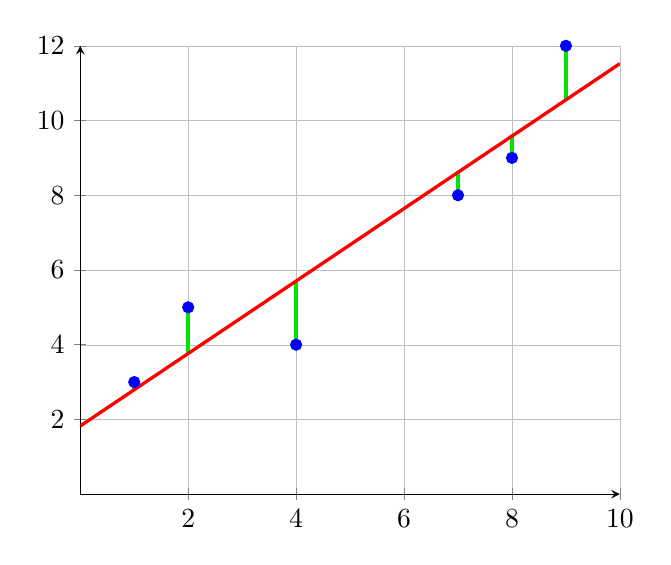
\begin{tikzpicture}
    \begin{axis}[
        axis lines=middle,
        %axis equal,  % somehow is dependent of the size of the box
        xmin=0, xmax=10,
        ymin=0, ymax=12,
        grid=both,
        grid style={line width=.1pt, draw=gray!50}
    ]
    \addplot [color=green!90!black,ultra thick] coordinates {(1,3) (1,2.793)};
    \addplot [color=green!90!black,ultra thick] coordinates {(2,5) (2,3.763)};
    \addplot [color=green!90!black,ultra thick] coordinates {(4,4) (4,5.702)};
    \addplot [color=green!90!black,ultra thick] coordinates {(7,8) (7,8.611)};
    \addplot [color=green!90!black,ultra thick] coordinates {(8,9) (8,9.581)};
    \addplot [color=green!90!black,ultra thick] coordinates {(9,12) (9,10.550)};
    \addplot [only marks, color=blue]%
    table[row sep=crcr] {
    1 3 \\
    2 5 \\
    4 4 \\
    7 8 \\
    8 9 \\
    9 12 \\
    };
    \addplot [domain=0:10, red, very thick] {1.824 + 0.970*x};
    \end{axis}
    \end{tikzpicture}
  
  \column{.5\textwidth}
  \bigskip
  
  We want a line of the form $y=\beta_0 + \beta_1 x$.
  \bigskip
  
  \pause
  Which line \alert{best fits} the data?
  \medskip
  
  We want to minimize the sum of squares
  \[
    \sqrt{\sum_{i=1}^n \bigg( \blue{y_i} - (\red{\beta_0 + \beta_1 x_i}) \bigg)^2 }.
  \]
  \qquad $\blue{y_i} - (\red{\beta_0 + \beta_1 x_i})$ is called the \green{residual}.
  \bigskip
  
  \pause
  \mbox{Can we formulate as a least-squares problem?}
  
  \centering \alert{Yes!}
  \end{columns}
\end{frame}


\begin{frame}{Best-Fit Line}
  \begin{columns}[T]
  \column{0.33\tw}
  We would like to solve:
  \begin{align*}
  y_1 &= \alert{\beta_0} + \alert{\beta_1} x_1 \\
  y_2 &= \alert{\beta_0} + \alert{\beta_1} x_2 \\
  y_3 &= \alert{\beta_0} + \alert{\beta_1} x_3 \\
      & \ \ \vdots  \\
  y_n &= \alert{\beta_0} + \alert{\beta_1} x_n \\ 
  \end{align*}

  \column{0.33\tw}
  \onslide<2->{
  As a matrix equation:
  \[ \begin{bmatrix} y_1 \\ y_2 \\ \vdots \\ y_n \end{bmatrix} = 
  \begin{bmatrix} 1 & x_{1} \\ 1 & x_{2} \\ \vdots & 
  \vdots \\ 1 & x_{n} \end{bmatrix} \begin{bmatrix} \alert{\beta_0} \\ \alert{\beta_1} \end{bmatrix} \]

  \[ \y = A \alert{\boldsymbol\beta} \]
  }
  
  \column{0.33\tw}
  \begin{center}
  \includegraphics[width=0.99\tw]{images/fig-residuals.png}
  \end{center}
  \end{columns}
  \vspace*{-1em}
  
  \pause\pause
  \bi
  \ii $A$ is called the \blue{model matrix} (or design matrix).
  \ii $\y$ is the vector of \blue{observed responses}.
  \ii $\boldsymbol\beta$ is the vector of \blue{regression coefficients}.
  \ei
  \medskip

  Computing the \alert{least-squares} solution of $\y = A \boldsymbol\beta$ is equivalent to finding
  values for the regression coefficients $\beta_0$ and $\beta_1$ that minimize the \green{sum of square residuals}.
\end{frame}


\begin{frame}{Example}
  \medskip
  
  Suppose we have data $(1,3),(2,5),(4,4),(7,8),(8,9),(9,12)$.
  What is the \alert{best-fit} line?
  
  \begin{columns}[T]
  \column{.3\textwidth}
    \bigskip
    
    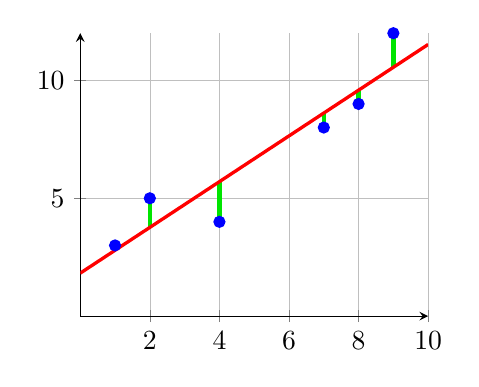
\begin{tikzpicture}
    \begin{axis}[
        width=6cm,
        axis lines=middle,
        %axis equal,  % somehow is dependent of the size of the box
        xmin=0, xmax=10,
        ymin=0, ymax=12,
        grid=both,
        grid style={line width=.1pt, draw=gray!50}
    ]
    \addplot [color=green!90!black,ultra thick] coordinates {(1,3) (1,2.793)};
    \addplot [color=green!90!black,ultra thick] coordinates {(2,5) (2,3.763)};
    \addplot [color=green!90!black,ultra thick] coordinates {(4,4) (4,5.702)};
    \addplot [color=green!90!black,ultra thick] coordinates {(7,8) (7,8.611)};
    \addplot [color=green!90!black,ultra thick] coordinates {(8,9) (8,9.581)};
    \addplot [color=green!90!black,ultra thick] coordinates {(9,12) (9,10.550)};
    \addplot [only marks, color=blue]%
    table[row sep=crcr] {
    1 3 \\
    2 5 \\
    4 4 \\
    7 8 \\
    8 9 \\
    9 12 \\
    };
    \addplot [domain=0:10, red, very thick] {1.824 + 0.970*x};
    \end{axis}
    \end{tikzpicture}
  
  \column{.5\textwidth}
  \medskip
  
  We want a least-squares solution of $\y=A\boldsymbol\beta$.
  \[
    \small
    \begin{bmatrix} 3 \\ 5 \\ 4 \\ 8 \\ 9 \\ 12 \end{bmatrix}
    =
    \begin{bmatrix}
      1 & 1 \\
      1 & 2 \\
      1 & 4 \\
      1 & 7 \\
      1 & 8 \\
      1 & 9
    \end{bmatrix}
    \begin{bmatrix} \beta_0 \\ \beta_1 \end{bmatrix}.
  \]
  \pause
  We solve the \alert{normal equations} by computing
  
  \hspace*{3em} $\boldsymbol\beta =(A^T A)^{-1} A^T \y = 
    \begin{bmatrix} 1.824 \\ 0.970 \end{bmatrix}$.
  \smallskip
  
  So $y=1.824 + 0.970x$ is the \alert{best-fit line}.
  \end{columns}
  \bigskip
  
  \pause
  We can quantify the \blue{error} by $\y = A\boldsymbol\beta + \boldsymbol\varepsilon = \hat\y+ \z$, $\|\z\| \approx 2.699$.
\end{frame}


\begin{frame}{Predicting Wealth Based on Literacy Rate}

  {\small Data scientists often begin with a simple model, and then determine whether predictions increase when new predictors are added. Let's first consider the following potential relationship:}

  {\small
  \bi
  \ii Let $y$ denote the Gross Domestic Product (GDP) per capita of a country (in thousands of dollars).
  \ii Let $x_{1}$ denote the literacy rate of the country's population (as a percentage).
  \ii We collect a dataset that consists of $n$ observations.
  \ii Based on our data, what is the best model of the form $y = \beta_0 + \beta_1 x_1$?
  \ei
  }

  \vspace{-0.1in}

  \begin{columns}[T]

  \column{0.33\tw}

  \begin{align*}
  2.079 &= \alert{\beta_0} + \alert{\beta_1} (31.4) \\
  13.440 &= \alert{\beta_0} + \alert{\beta_1} (98.1) \\
  11.324 &= \alert{\beta_0} + \alert{\beta_1} (81.4) \\
  & \vdots  \\
  3.537 &= \alert{\beta_0} + \alert{\beta_1} (88.7) \\ 
  \end{align*}

  \column{0.33\tw}

  \[ \begin{bmatrix} 2.07 \\ 13.44 \\ 11.324 \\ \vdots \\ 3.537 \end{bmatrix} = \begin{bmatrix} 1 & 31.4 \\ 1 & 98.1 \\ 1 & 81.4 \\  \vdots &  \vdots \\ 1 & 88.7 \end{bmatrix} \begin{bmatrix} \beta_0 \\ \beta_1 \end{bmatrix} \]

  \column{0.33\tw}

  \vspace{-0.15in}

  \begin{center}
  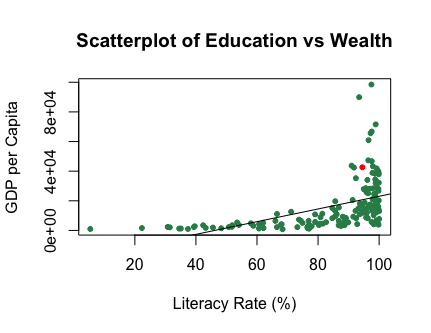
\includegraphics[width=0.97\tw]{images/fig-edu-gdp.png}
  \end{center}

  \end{columns}
\end{frame}


\begin{frame}{Interpreting the Results}
  Let's imagine that we randomly select four countries record the most recent data for each country's GDP per capita and literacy rate. \alert{$ \widehat{\texttt{Wealth}} = -1.938 + 0.126( \texttt{Education})$} 

  \[ A= \begin{bmatrix} 1 & 31 \\ 1 & 98 \\ 1 & 81 \\ 1 & 89 \end{bmatrix}  \quad \mbox{and} \quad \mathbf{y} =\begin{bmatrix} 2 \\ 13 \\ 11 \\ 4 \end{bmatrix} 
  \onslide<2->{
  \quad A^T A = \begin{bmatrix} 1 & 1 & 1 & 1 \\ 31 & 98 & 81 & 89 \end{bmatrix}  \begin{bmatrix} 1 & 31 \\ 1 & 98 \\ 1 & 81 \\ 1 & 89 \end{bmatrix} = \begin{bmatrix}4 & 299 \\ 299 & 25,\!047 \end{bmatrix}} \]

  \pause
  For the least-squares solution to $A \boldsymbol\beta = \y$,
  we solve the normal equations $A^T A \boldsymbol\beta = A^T \y$:

  \[ \boldsymbol\beta = \begin{bmatrix} \beta_0 \\ \beta_1 \end{bmatrix}  = \left( \begin{bmatrix}4 & 299 \\ 299 & 25,\!047 \end{bmatrix} \right)^{-1}  \begin{bmatrix} 1 & 1 & 1 & 1 \\ 31 & 98 & 81 & 89 \end{bmatrix} \begin{bmatrix} 2 \\ 13 \\ 11 \\ 4 \end{bmatrix} \approx \begin{bmatrix} -1.938 \\ 0.126 \end{bmatrix} \]
\end{frame}


\begin{frame}{Fitting a Model for Predicting Wealth of a Nation}
  Let's imagine that we randomly select four countries record the most recent data for each country's GDP per capita and literacy rate. 

  \begin{columns}[T]
  \column{0.5\tw}
  \alert{$ \widehat{\texttt{Wealth}} = -1.938 + 0.126( \texttt{Education})$} 
  \ms

  {\small
  \bb
  \ii  The literacy rate in the United States in 2021 is approximately 80\%. Based on our model predict the GDP per capita of the US? (Note the actual value is $\$69,\!734$.)
  \ii Interpret the practical meaning of the slope and vertical intercept of the linear model.
  \ee }

  %\begin{tabular}{l|c|c}
  %Country & GDP per capita & Literacy Rate \\
  %\hline
  %A & 2 & 31 \\
  %B & 13 & 98 \\
  %C& 11 & 81 \\
  %D & 4 & 89 \\
  %\end{tabular}

  \column{0.5\tw}
  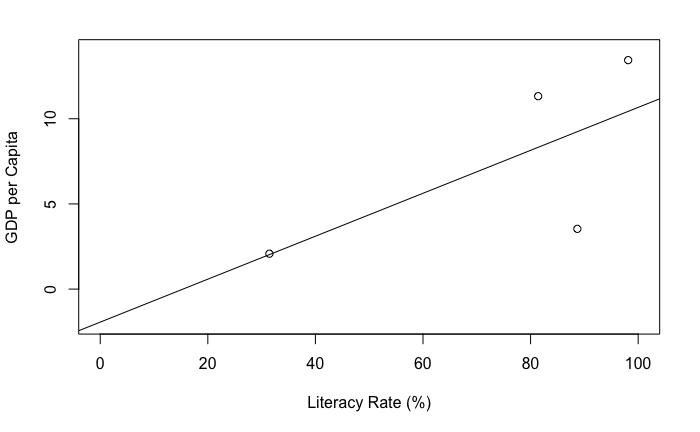
\includegraphics[width=0.95\tw]{images/fig-sample-wealth.png}
  \end{columns}
\end{frame}


\begin{frame}{Multiple Regression}
  \smallskip
  
  We can include other factors and also fit them.
  \medskip

  {\small
  \begin{tabular}{c|c|c|c}
  Wealth & Literacy & Life Exp & Area\\
  \hline
  2 & 31 & 65 & 653\\
  13 & 98 & 79 & 27\\
  11 & 81 & 77 & 2381\\
  4 & 89 & 61 & 387\\
  \end{tabular} \ \ \ \ \ $\dsty A = \begin{bmatrix} 1 & 31 & 65 & 653 \\ 1 & 98 & 79 & 27 \\ 1 & 81 & 77 & 2381 \\ 1 & 89 & 61 & 387 \end{bmatrix}$, \ \ \  $\dsty \y = \begin{bmatrix} 2 \\ 13 \\ 11 \\ 4 \end{bmatrix}$. }

  We wish to find the regression coefficients $\beta_0, \beta_1, \beta_2$, and $\beta_3$ that will give us the best fitting model of the form
  \[ \texttt{wealth} = \alert{\beta_0} + \alert{\beta_1} (\texttt{Literacy}) + \alert{\beta_2} (\texttt{LifeExp}) + \alert{\beta_3} (\texttt{Area}) + \colorg{\epsilon}. \]
  
  \pause
  Solving the normal equations, we obtain
  \[ \small \alert{\boldsymbol\beta = 
  \begin{bmatrix} \beta_0 \\ \beta_1 \\  \beta_2 \\  \beta_3 \end{bmatrix}} 
  = (X^TX)^{-1} X^T \mathbf{y} \approx
  \begin{bmatrix} -30.458 \\ 0.067 \\ 0.467 \\ 0.00003 \end{bmatrix} \]

  \[ \widehat{\texttt{wealth}} = \alert{-30.458} + \alert{0.067 } (\texttt{Literacy}) + \alert{0.467} (\texttt{LifeExp}) + \alert{0.00003} (\texttt{Area})  \]
\end{frame}


\begin{frame}{Fitting Other Models}
  \bigskip

  We call any model which is linear in the coefficients $\beta$'s a \blue{linear model}.
  \medskip

  For example:

  \bi
  \ii $y = \beta_0 + \beta_1 x_1 + \beta_2 x_2 $ includes two factors. \smallskip
  \ii $y = \beta_0 + \beta_1 x_1 + \beta_2 x_2 + \beta_3 x_1 x_2$ includes an interaction term. \smallskip
  \ii $y = \beta_0 + \beta_1 x + \beta_2 x^2$ is a linear model that includes a second-order term. \smallskip
  \ei
\end{frame}


\begin{frame}{Fitting a Quadratic Polynomial}
  \medskip
  
  Consider a ball thrown from $(0,0)$.  The height is measured at the following distances:
  
  \centering $(1,3), (10,8), (15,6)$.  Where do we predict the ball will hit the ground?
  
  \begin{columns}[T]
  \column{.5\textwidth}
    
  \onslide*<1-2>{%
    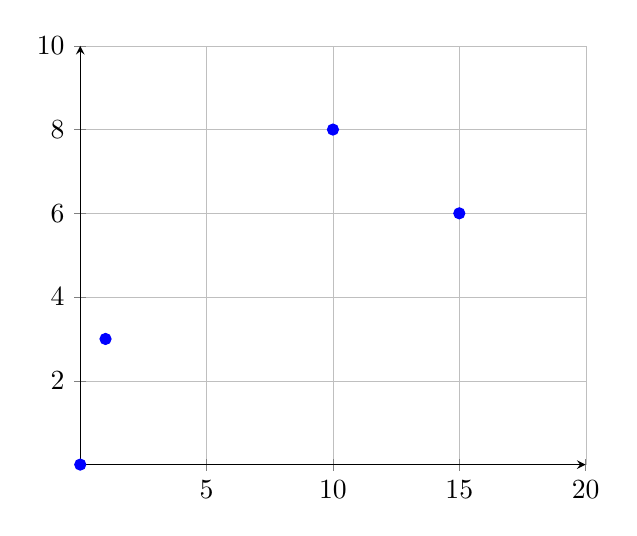
\begin{tikzpicture}
    \begin{axis}[
        width=8cm,
        axis lines=middle,
        %axis equal,  % somehow is dependent of the size of the box
        xmin=0, xmax=20,
        ymin=0, ymax=10,
        grid=both,
        grid style={line width=.1pt, draw=gray!50}
    ]
    \addplot [only marks, color=blue]%
    table[row sep=crcr] {
    0 0 \\
    1 3 \\
    10 8 \\
    15 6 \\
    };
    %\addplot [domain=0:20, red, very thick] {0.691 + 1.567*x -0.0813*x^2};
    \end{axis}
    \end{tikzpicture}%
    }\onslide*<3->{%
    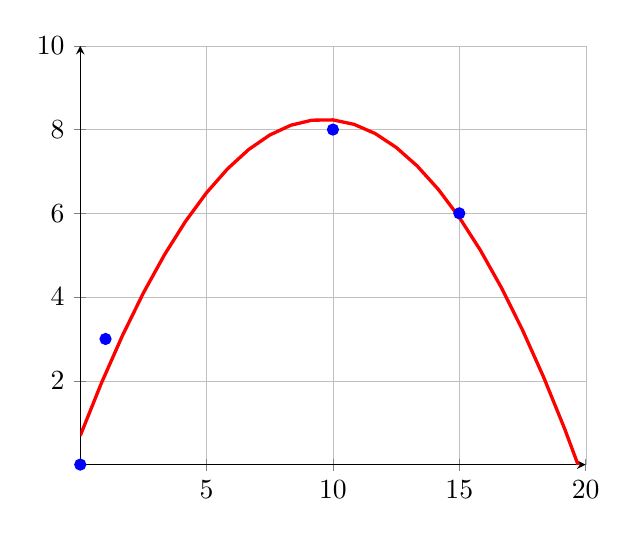
\begin{tikzpicture}
    \begin{axis}[
        width=8cm,
        axis lines=middle,
        %axis equal,  % somehow is dependent of the size of the box
        xmin=0, xmax=20,
        ymin=0, ymax=10,
        grid=both,
        grid style={line width=.1pt, draw=gray!50}
    ]
    \addplot [only marks, color=blue]%
    table[row sep=crcr] {
    0 0 \\
    1 3 \\
    10 8 \\
    15 6 \\
    };
    \addplot [domain=0:20, red, very thick] {0.691 + 1.567*x -0.0813*x^2};
    \end{axis}
    \end{tikzpicture}%
  }
  
  \column{.5\textwidth}
  \medskip
  
  {\small
  \pause
  We use a model of $y=\beta_0 + \beta_1 x + \beta_2 x^2$.
  \[
    \small
    \begin{bmatrix} 0 \\ 3 \\ 8 \\ 6 \end{bmatrix}
    =
    \begin{bmatrix}
      1 & 0 & 0^2 \\
      1 & 1 & 1^2 \\
      1 & 10 & 10^2 \\
      1 & 15 & 15^2
    \end{bmatrix}
    \begin{bmatrix} \beta_0 \\ \beta_1 \\ \beta_2 \end{bmatrix}.
  \]
  \pause
  We solve the \alert{normal equations} by computing
  
  \hspace*{3em} $\boldsymbol\beta =(A^T A)^{-1} A^T \y = 
    \begin{bmatrix} 0.691 \\ 1.567 \\ -0.0813 \end{bmatrix}$.
  \smallskip
  
  So ${\footnotesize y=0.691 + 1.567x -0.0813x^2}$ is the \alert{best fit}.
  \bigskip
  
  \pause
  Using the quadratic formula, height $=0$ at \green{$19.703$}.
  }
  \end{columns}
  
  
\end{frame}

\end{document}
